\documentclass[11pt,a4paper]{report}

% Aberstwyth dissertation LaTeX Template
% Authors: Dr. Hannah Dee (hmd1@aber.ac.uk), Neil Taylor (nst@aber.ac.uk)
% This has been adapted from the Leeds Thesis template and the 
% Group Project template for Computer Science in Aberystywth University.
% 
% All comments and suggestions welcome.
%
% Template designed to be used with pdflatex: it may need alteration to
% run with a different LaTeX engine
%
% Note - this is offered as a starting point for your work. You are not 
% required to use this template and can choose to create your own document 
% without it. 

% To build document on the unix command line, run four commands:
 
% pdflatex dissertation
% bibtex dissertation
% pdflatex dissertation
% pdflatex dissertation

% you will end up with dissertation.pdf 
\usepackage{mmp}
\usepackage{listings}

% the following packages are used for citations - You only need to include one. 
%
% Use the cite package if you are using the numeric style (e.g. IEEEannot). 
% Use the natbib package if you are using the author-date style (e.g. authordate2annot). 
% Only use one of these and comment out the other one. 
\usepackage{cite}
%\usepackage{natbib}

% Use the following to selectively exclude chapters
%\includeonly{cover,abstract,acknowledge,declare,chapter1,chapter2}

\begin{document}

% all of the include directives below refer to tex files
% so 
\title{Building an Online Resource for {\it Candida tropicalis}}

% Your name
\author{Owen Garland}

% Your email 
\authoremail{owg1@aber.ac.uk}

\degreeschemecode{G600} %e.g. G400 
\degreeschemetitle{Software Engineering} % e.g. Computer Science
\degreetype{BEng}

\modulecode{CS39440} % i.e. CS39440, CC39440, CS39620
\moduletitle{Major Project} % i.e. Major Project or Minor Project

\date{\today} % i.e. the date of this version of the report

\status{Draft} % Use draft until you create the release version. Then, change this to Release.
\version{1.0}

%The title and name of your supervisor.
\supervisor{Dr.\ Wayne Aubrey} 

%The email for your supervisor. 
\supervisoremail{waa2@aber.ac.uk}

\maketitle
 includes cover.tex - to change the content,
% edit the tex file

\pagenumbering{roman}

% This is the front page

\title{Building an Online Resource for {\it Candida tropicalis}}

% Your name
\author{Owen Garland}

% Your email 
\authoremail{owg1@aber.ac.uk}

\degreeschemecode{G600} %e.g. G400 
\degreeschemetitle{Software Engineering} % e.g. Computer Science
\degreetype{BEng}

\modulecode{CS39440} % i.e. CS39440, CC39440, CS39620
\moduletitle{Major Project} % i.e. Major Project or Minor Project

\date{\today} % i.e. the date of this version of the report

\status{Draft} % Use draft until you create the release version. Then, change this to Release.
\version{1.0}

%The title and name of your supervisor.
\supervisor{Dr.\ Wayne Aubrey} 

%The email for your supervisor. 
\supervisoremail{waa2@aber.ac.uk}

\maketitle
                        

% Set up page numbering
\pagestyle{empty}

% declarations of originality 
\thispagestyle{empty}

%%%
%%% You must sign the declaration of originality. 
%%%
%%% You are submitting this electronically. Therefore, to sign, you 
%%% type your name and date to replace the .... characters. 
%%%
\begin{center}
    {\LARGE\bf Declaration of originality}
\end{center}

I confirm that:

\begin{itemize}
\item{This submission is my own work, except where 
clearly indicated.}

\item{I understand that there are severe penalties for Unacceptable Academic Practice, which can lead to loss of marks or even the withholding of a degree.}
 
\item{I have read the regulations on Unacceptable Academic Practice from the University's Academic Quality and Records Office (AQRO) and the relevant sections of the current Student Handbook of the Department of Computer Science.}
 
\item{In submitting this work I understand and agree to abide by the University's regulations governing these issues.}
\end{itemize}

\vspace{2em}
Name ............................................................  \\

\vspace{1em}
Date ............................................................ \\

%%% 
%%% We would like to make a selection of final reports available to students that take 
%%% this module in future years. To enable us to do this, we require your consent. You 
%%% are not required that you do this, but if you do give your consent, then we will have 
%%% the option to select yours as one of a number of reports as examples for other 
%%% students. If you would like to give your consent, then please include the following 
%%% text and type your name and date to replace the .... characters. 
%%% 
%%% If you do not wish to give your consent, please remove this from your report. 
%%%
\vspace{1em}
\begin{center}
    {\LARGE\bf Consent to share this work}
\end{center}

By including my name below, I hereby agree to this dissertation being made available to other students and academic staff of the Aberystwyth Computer Science Department.  

\vspace{2em}
Name ............................................................  \\

\vspace{1em}
Date ............................................................ \\


               

\thispagestyle{empty}

\begin{center}
    {\LARGE\bf Acknowledgements}
\end{center}

I would like to thank my supervisor Wayne Aubrey, for being incredibly supportive of this project, helping me to understand so much more about genetics and biology in general, as well as giving me lifts to go and meet the researchers, David Bryant and Abhishek Somani, who were also tremendously helpful and patient with all the questions I had. 
 % Acknowledgements
\thispagestyle{empty}

\begin{center}
    {\LARGE\bf Abstract}
\end{center}

Understanding data produced by next gen sequencing technologies is a difficult problem, not helped by a lack of well designed software and user experiences. 

Researchers at Aberystwyth University are looking into the possibly of modifying a species of yeast, \textit{Candida tropicalis}, to convert xylose into xylitol. 

If xylitol can be produced by \textit{C. tropicalis} it would provide a cheaper supply of the sugar, which has antibacterial properties, as well as a very low glycaemic index, making it suitable for people suffering from diabetes.

To do this they have sequenced the DNA of three species of yeast, \textit{C. tropicalis, C. shehate} and \textit{C. boidinii}, but now need an accessible and meaningful way to interact with the data produced.

Most genome database software is already over a decade old, and continue to use dated practices, and technologies. 

The aim for this project is to apply modern web development standards to this problem and produce a web site to display their data using NodeJS, with the data stored in a NoSQL database. 

The implementation of this database and website has shown that NoSQL is a viable approach to storing and viewing genomic information, especially for smaller genomes. However it does also acts as a proof of concept and provides a step stone for the building of a larger open source project that aims to accommodate larger genomes. 

Importantly it shows that modern technologies and approaches can have a meaningful benefit over the old monolithic solutions, especially in terms of producing high quality maintainable software.
                 % Abstract

\pagenumbering{roman}
\pagestyle{fancy}
\fancyhead{}
\fancyfoot[C]{\thepage}
\renewcommand{\headrulewidth}{0 pt}
\renewcommand{\chaptermark}[1]{\markboth{#1}{}}

\tableofcontents   
\newpage
\listoffigures
\newpage 
\listoftables
\newpage

% Set up page numbering
\pagenumbering{arabic}

\setchapterheaderfooter

% include the chapters
\chapter{Background \& Objectives}

This section should discuss your preparation for the project, including background reading, your analysis of the problem and the process or method you have followed to help structure your work.  It is likely that you will reuse part of your outline project specification, but at this point in the project you should have more to talk about. 

\textbf{Note}: 

\begin{itemize}
   \item All of the sections and text in this example are for illustration purposes. The main Chapters are a good starting point, but the content and actual sections that you include are likely to be different.
   
   \item Look at the document on the Structure of the Final Report for additional guidance. 
   
\end{itemize}

\section{Background}
Researchers at Aberystwyth University have been studying three species of yeast, \textit{Candida tropicalis}, \textit{Candida boidinii}, and \textit{Candida shehatae}. To study the genetics of these species, they have each had their genomes sequenced by Illumina sequencing machines. From that point the sequences of DNA that have been read are then assembled into contigs (contiguous DNA fragments). This process produces an accurate representation of the species DNA, which then can then be aligned to other better understood DNA and annotated as such.

Arabinose and Xylose are five carbon sugars ubiquitously found in plants such as grass, which can be used as a feedstock for industrial biotechnology. \textit{Candida tropicalis} is able to convert arabinose \& xylose into arabitol and xylitol respectively. Xylitol is a commercially valuable anti-bacterial foodgrade sugar use in the manufacture of chewing gum. However arabitol and xylitol are stereoisomers and cannot be easily separated. \textit{Candida boidinii} cannot metabolise arabinose, for an unknown reason, but does metabolise Xylose but at a much slower rate which is commercially in-viable.

Understanding at a genomic level why \textit{Candida boidinii} is unable to utilise arabinose and genetically modifying \textit{Candida tropicalis} to have the same phenotype, may enable \textit{Candida topicalis} to exclusively produce xylitol and not arabitol. One other exciting possibility is using it as a low glycaemic index table sugar that can be used by diabetics.

What was your background preparation for the project? What similar systems or research techniques did you assess? What was your motivation and interest in this project? 

\section{Analysis}
Taking into account the problem and what you learned from the background work, what was your analysis of the problem? How did your analysis help to decompose the problem into the main tasks that you would undertake? Were there alternative approaches? Why did you choose one approach compared to the alternatives? 

There should be a clear statement of the research questions, which you will evaluate at the end of the work. 

In most cases, the agreed objectives or requirements will be the result of a compromise between what would ideally have been produced and what was felt to be possible in the time available. A discussion of the process of arriving at the final list is usually appropriate.

\section{Research Method and Software Process}
You need to describe briefly the life cycle model or research method that you used. You do not need to write about all of the different process models that you are aware of. Focus on the process model or research method that you have used. It is possible that you needed to adapt an existing method to suit your project; clearly identify what you used and how you adapted it for your needs.

For the research-oriented projects, there needs to be a suitable process for the construction of the software elements that support your work. 

%\addcontentsline{toc}{chapter}{Development Process}
\section{Provided Data}
The data for this project was produced by a contracted researcher who had since moved onto another project. Because of this there was limited opportunity to talk with them about the data, how it was produced and what needed doing to it. Unfortunately, the data did not include any form of documentation, or annotation as to how it was produced, the only metadata available was the filenames. 

This lead to a lot of confusion as it wasn't immediately obvious what each bit of data was and what it meant. Examining the data and learning about the biology behind it took several weeks, and ascertaining what bits of data were actually relevant to the project took even longer. Eventually it was determined that for each species there were three files that would need to be incorporated into the project.

\begin{itemize}
  \item Raw assembled contigs of DNA, these would be used to find a genes position in the genome, and its surrounding bases. 
  \item Amino acid sequences that code for the proteins found using BLAST to align the assembled contigs against the NCBI non-redundant protein database, annotated with Gene Ontology ID's and protein function.
  \item Coding sequences, these are the nucleotide sequences that coded for the amino acid sequences. 
\end{itemize}

Linking this data to the Candida Genome Database (CGD) was a key bit of information that was missing. To do this the annotated proteins\cite{albicans} for \textit{C. albicans} were downloaded, then turned into a reference database with Diamond. With this the three species could then have their coding sequences aligned against \textit{C. albicans} to produce accession ID's from the Candida Genome Database. The script that performed this step is included in the project as \texttt{run\_diamond.sh}.

Several sets of data were then required to map these proteins to the Candida Genome Database, which would allow the researchers to easily compare the genes to well annotated species. First was a file of Gene Ontology\cite{geneontology} annotations for all the proteins stored in the Candida Genome Database\cite{cgd-proteins}. This file conveniently also stores all the accession ID's for those proteins. This is what was used to map the alignment results to the Candida Genome Database, by selecting the accession ID from the Diamond alignment results, and looking that up in this data set, the Candida Genome ID was able to be found.

In addition to this was a mapping file that mapped Candida Genome Database ID's to UniProt\cite{uniprot} ID's. With a small JavaScript script and some manual cleaning with a text editor, a complete mappings file was able to be produced in JSON, ready to be read in by the importation script. This allows for genes found to be linked to other well known genes in the Candida Genome Database and UniProt.

\chapter{Software Design, Implementation and Testing}

\section{Requirements}
There are two main components to the software being developed for this project. The first is the manipulation of the data into a database, and the second is a web front end for the data to be accessed via. 

\subsection{Database}
The database has to store the following information for each hit from the alignment with \textit{C. albicans}:

\begin{itemize}
  \item ID of the hit that was found when the species coding sequences have been aligned with \textit{C. albicans}.
  \item Species it came from.
  \item The gene name and ID from Candida Genome Database.
  \item UniProt ID.
  \item Contig of raw DNA.
  \item Coding sequence of nucleotides.
  \item Protein sequence that the coding sequence codes for.
  \item Annotations from NCBI nr database to provide a description of the proteins.
  \item A list of Gene Ontology\cite{geneontology} ID's for the protein.
  \item If it can be found, the positions of the start and end of the coding sequence in the raw contig. 
\end{itemize}

From these requirements it is clear there are a few pieces of data that need to be extracted from the data that has been collated. For each alignment with \textit{C. albicans} the protein sequence and GO annotations need to found, the coding sequence that was used in the alignment and the contig that it came from. In addition to this, the metadata about the genes such as the name and ID's need to be read from the mapping file that was created earlier. 

The final bit of data that needs to be added is the position of the coding sequence in the contig. An algorithm will have to be developed to detect this.

\subsection{Website}
The website will only have a few funcitonal requirements: 

\begin{enumerate}[label=FR\arabic*]
  \item Display each record in the database in an easy to read manner. 

    The first requirement, is that each document in the database can be accessed, and presented to the user. It will have to display all of the fields of the document without overwhelming the user, this is a risk as some of the sequences are very large. Links to other databases such as the GeneOntology database, and UniProt database will have to be made into hyperlinks for the user to easily navigate to the relevant information for the found gene. 

  \item Highlight coding sequence in contig if possible.

    Visually representing the coding sequence inside of the raw assembled contig, is helpful for researchers to see the surrounding bases up and down stream of the coding sequence. It also allows them to see the full coding sequence with any introns (non-coding regions of bases) included. 

  \item Copy coding sequence and +/- a user defined number of bases to the clipboard.

    The user should also be able to copy the coding sequence to their clipboard, for use in other applications. They should also be able to select a number of bases to be copied that surround the coding sequence. 

  \item Search the database for a gene, by name, description, ID, or even by nucleotide sequence. 

    The search functionality is the main feature of the site as it is what takes the previously difficult to use data, and makes it truly accessible. 
\end{enumerate}


\section{Build Process}
  One of the first things that was setup for this project was the build process. This doesn't take long to setup but provides a huge benefit for the rest of the project. It helps to reduce errors and speed up the process of deployment and testing.

  \subsection{Development Environment}
    This project will be developed on an Arch Linux system, as it will only ever be ran on a Linux host this isn't an issue, as the production hosts' architecture will match the development one. 

    All of the code and LaTeX form the report will be written with the Vim text editor, which has been configured to have many optimisations to this workflow. The full Vim configuration that was used can be found here\cite{vimrc}.

  \subsection{Code Style}
  For this project the Clock Limited code standard\cite{clockstandard} will be followed. This has a few key variations to typical Javascript. 

  \begin{itemize}
    \item Semicolons are not required in JS, so they are not used to denote end of line.
    \item Strings are encapsulated with single quotes, not double. 
    \item Comma first\cite{commafirst} listing of variables, objects and arrays.
    \item No commenting, to avoid confusion, encourage descriptive naming and reduce file length.
  \end{itemize}

  These rules ensure that the code written is clean and easy to read, something that is crucial for producing high quality and easily maintainable code. 

  \subsection{Version Control}
    This project is being entirely tracked with Git version control. This is to ensure that all of the work is backed up to a remote repository, with an easily accessible history. It also allows for branching of the project to test out experimental features or bug fixes. The project is remotely hosted on Github\cite{github} for remote backup and access via multiple hosts. Github is also widely supported by third party integrations, something that will be utilised quite extensively, in this build and deployment process tool chain.


  \subsection{Test Suite}
  When pushing code to Github, a module called Husky\cite{husky} will run the test suite on the developers local machine.

    The test suite is set up to first clean the project of old builds and coverage reports, then run ESlint\cite{eslint}. This will scan the entire codebase for files that do not adhere to the code style. This means that any badly formatted code will cause an error and prevent the code from being pushed until the issues are fixed.

    After the linting check, the test suite will use Mocha\cite{mocha} to run all of the JavaScript test files that are in the project. If any of the assertions made in the test files fail, the project will not be pushed. 

    Once the test's have been ran Istanbul\cite{istanbul} will provide a coverage report, that will show to the user the percentage of tested code that has been covered by the assertions. After this the code can finally be pushed to Github. 
    
  \subsection{Continuous Integration}
    Once the code has been pushed to Github, a hook on Github will trigger Travis CI\cite{travis} to clone down the latest version of the code to it's servers and run the test suite again on it's own server. This is very useful as occasionally developers can bypass Husky to push code, or have something setup in their system that isn't defined in the application that causes test to pass on their system but not when the application is built from scratch. The CI test will expose any bugs that arise from these situations and prevent the code being deployed to the testing server. 

    Once those tests are successful, it will send the coverage report generated by Istanbul to another third party service called Codecov\cite{codecov}. This tracks the test coverage over time and provides interactive charts highlighting areas that need more test coverage. 

\begin{figure}[H]
\begin{center}
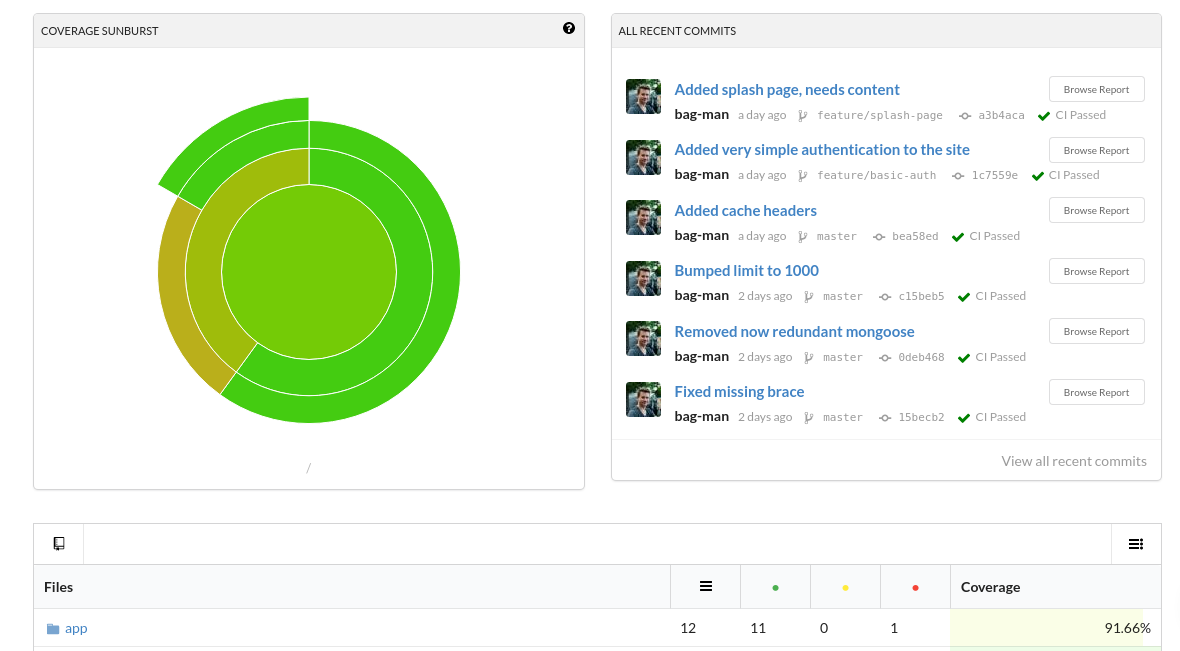
\includegraphics[scale=0.3]{codecov}
\caption{Codecov interactive coverage report}
\end{center}
\end{figure}


  \subsection{Deployment}
  If the tests pass on Travis CI, a Github hook will then activate the deployment. The project is setup to use Heroku\cite{heroku}, and to build on successful CI results. This means that when code is pushed to the master branch, it will automatically be deployed to their service. This is excellent for development as it allows changes made to the system to be almost immediately reflected on the live website. The only drawback of Heroku is that this project is using their free offerings which only allow 500MB's of database storage, which means that anything larger than that will be truncated. 

  The benefits of this build process are clear, firstly code is automatically deployed, which saves time as deployments don't have to be done manually, as well as encouraging regular client feedback. However the main advantage is that before the deployment the code will have had the test suite ran on it twice, once on the developers local machine and then again on a brand new build on the CI service. This means that any mistakes are caught before they are put into production and the developer is notified of these issues so they can't be avoided. 


\section{Design}
% You should concentrate on the more important aspects of the design. It is essential that an overview is presented before going into detail. As well as describing the design adopted it must also explain what other designs were considered and why they were rejected.
% 
% What design will be used?
% 
% What implementation issues are there and what testing is used? 
% 
% Even though a research project is investigating specific research questions, it is still necessary for you to discuss the software that you develop. Research has a habit of generating bits of software that can exist for several years and need future modification. Therefore you need to be able to discuss the technical issues as well as the research approach. 

\subsection{Choice of Database Technology}
The first stage in designing this system was to decide upon what database technology would be used for the data store. In the Analysis section the merits and disadvantages of NoSQL and SQL solutions were highlighted in generic terms. For this project there is a focus on using modern web development technologies, and MongoDB (A NoSQL database solution) fits this well, as it stores data based on use case. 

In this project there will only be one set of data to be stored, the list of genes and their various related data. From the users perspective they will only be interacting with this set of data, they will never be trying to combine a gene with another dataset for example. 

If this data was stored in a relational system like PostgreSQL, then there would need to be several tables for shared data, to store it in a normalised form. For example, there would be a contig table and each gene would store a link to the contig that it was from. This means that when a user requests to view a gene the database will have to perform a join between the gene table and the table storing the contig to retrieve all of the relevant information. This makes it harder to develop and maintain the database, as the relations between the datasets have to be considered throughout the project. 

This would be advantageous if the data was going to be updated frequently, as a piece of data only needs to be updated once, as it is only stored once. However as this project is effectively read only, the data is never going to change, this isn't an issue with MongoDB.

This choice was also influenced by the choice of server side language, which for this project will be NodeJS. 

\subsection{Choice of Server Side Technology}
NodeJS was chosen for several reasons, firstly as both server side and client side portions of the code are written in JavaScript, it is easier to develop, since you are working with one unified language. 

It also works very well with MongoDB as, MongoDB represents it's data as JSON objects, which are native to JavaScript, this makes querying and operating on data returned via MongoDB much easier, as it is already in a format native to the language. 

NodeJS has a very good packaging system, called Node Package Manager (npm), the npm repository has access to the largest collection of software packages, as well as being very easy to use and maintain package lists thanks to the package.json file, which is automatically updated when new modules are used. 

JavaScript has historically been looked down on due in part to it's syntax and type system, however with the latest stable specification\cite{es6} (ES6) of the language a lot of these issues have been addressed. 

As outlined in Ioannis K. Chaniotis et al's paper, `Our study concludes that Node.js offers client-server development integration, aiding code reusability in web applications, and is the perfect tool for developing fast, scalable network applications.'\cite{node-perf}

In addition to this I have a lot of prior experience with the language and ecosystem, which reduces the barriers to development that learning a new language would create. 

\subsubsection{Nodestack}
As well as NodeJS the project will also be utilising a set of boilerplate code called \cite{nodestack}. This code helps to setup a project and provides many extra features to the basic NodeJS stack. 

\subsubsection*{Node JS / ES6}

"Node.js is a JavaScript runtime built on Chrome's V8 JavaScript engine. Node.js uses an event-driven, non-blocking I/O model that makes it lightweight and efficient. Node.js' package ecosystem, npm, is the largest ecosysubsubsection*{of open source libraries in the world."\cite{node-org}
    Since Node \textgreater4.0 it has supported the ES6 standard, which provides a lot of syntactic sugar, and makes the formatting of the code a lot easier to read and write. 
    \subsubsection*{Webpack}
    
    Webpack is a module bundler that allows for easy packaging of client side javascript. It allows the client side javascript to be written in ES6, then when built it will transpile the ES6 code into more widely supported ES2015 code, minify it for efficient, and package it into one single file. This means that the code can be written in a nicely organised manner across multiple files in ES6, and then reduced to one small file for actual usage. 

    \subsubsection*{Mongoose}

    Mongoose is an Object Data Manager, it allows developers to define schema's and validation for their data objects as well as extensible models for those objects. This makes interactions with MongoDB a lot simpler, as well as easy enforcement of validation rules.

    \subsubsection*{Pug}

    Pug is an HTML templating language that allows developers to write HTML with dynamic variables from the server side, and include some logic elements. The main benefit is that it has a much cleaner syntax than HTML so it is a lot easier to read and write. 

    \subsubsection*{Stylus}

    Stylus is an expressive CSS language that, like Pug and ES6, improves the syntax of CSS by minimising unnecessary elements. It has many other advantages over CSS, although for this project they aren't likely to be utilised as the front end design work of this project will be minimal. 

    \subsubsection*{Bootstrap}

    Bootstrap is a CSS and JS framework that is aimed at making responsive websites easier to write. With the addition of bootstrap to the project adapting the front end to work on mobile will be minimal. It also adds useful features for laying out the page and some attractive default CSS. 

Using this boilerplate will save a huge amount of time in development as the basic framework of the web application is already laid out, so the development time can be focussed on developing software to meet the functional requirements rather than investing time in setting up a good web framework. 

For more detail on how the boiler plate works, you can read the guide here: \url{http://blog.owen.cymru/nodejs-es6-boiler-plate/}

\subsection{Database Import}
To import the genenomic data into the database from the fasta file format, a script will be written that will use a npm module called fasta2json\cite{fasta2json} to read the fasta files into JSON format. 

From there it will use the blast results generated by the diamond script to look up the cotnig, coding sequence, and amino acid sequence (protein) for each of the blast results. 

It will also compare the hit ID with the mappings file that was produced to get the ID's for the equivalent Uniprot and Candida Genome Database hits, if they are available. 

That data will then be inserted into MongoDB, and an index built on the searchable fields. This index will allow for a very fast and efficient search for the key fields that will be searched for in the database, description, gene name and ID's.

\begin{lstlisting}[caption=The database schema that will represent the hit object]
  { id: Schema.ObjectId
  , hitid: String
  , species: String
  , name: String
  , cgdid: String
  , uniprot: String
  , contig: 
    { head: String
    , seq: String 
    }
  , codingseq: 
    { head: String
    , seq: String 
    }
  , protein: 
    { head: String
    , seq: String
    , goids: [String]
    , desc: String 
    }
  , codingRange: 
    { start: Number
    , end: Number
    , fail: Boolean 
    }
  }
\end{lstlisting}

    
\subsection{Website Architecture}
As the application only has one data object to model, the architecture isn't that complex. However it is still beneficial to follow good design principles which is why a traditional Model View Controller (MVC) design pattern\cite{mvc} was followed. 

The MVC design pattern allows for each data object that is being modelled to have three components, a model which defines the data's structure and it's functionality, a controller that is how the application interacts with that model, and finally a view, which is what is displayed to the user and how they interact with the model. For example a user may click on a gene, which sends a request to the controller, the controller then requests that gene from the model, which in turn updates the view, that the user can then see the gene that they had selected. 

Abstracting the functionality of the project out into these three components allows for the development to be a lot easier to manage and work with, than having one monolithic class to handle the entire functionality of a data object. 

There will only be two routes in the application, one to the home page, which will simply display a splash page with some user information on, and another route handles searching and viewing genes, this will be done by have a URL parameter for the gene ID in the database. 

If this is present then the view to display a gene in full will be displayed to the user. If it isn't present then a search must have been performed and the query string in the URL will provide the options for the search. A search will return just a few key fields for each search results and then display the results in a list.   

When viewing a gene, the coding sequence will have to be highlighted inside of the contig, to do this the coding range that was determined when the data was imported will be used to select the substring. 

As the coding sequences are stored in the database in only one compliment, there will be a reverse compliment button to reverse the compliment of the coding sequence. This is useful if the coding sequence is highlighted in the contig as the reverse compliment, it will allow the users to check that the data is correct. 

\subsection{User Interface}
Before building the user interface for this project, I examined several other similar sites to see what information they were displaying and how it was laid out. The first was the Candida Genome Database\cite{cgd} and it's "Locus" page. It lists column headings on the left, and the the infromation on the right. This design is easy to read and doesn't clutter up the page too much.

\begin{figure}[H]
\begin{center}
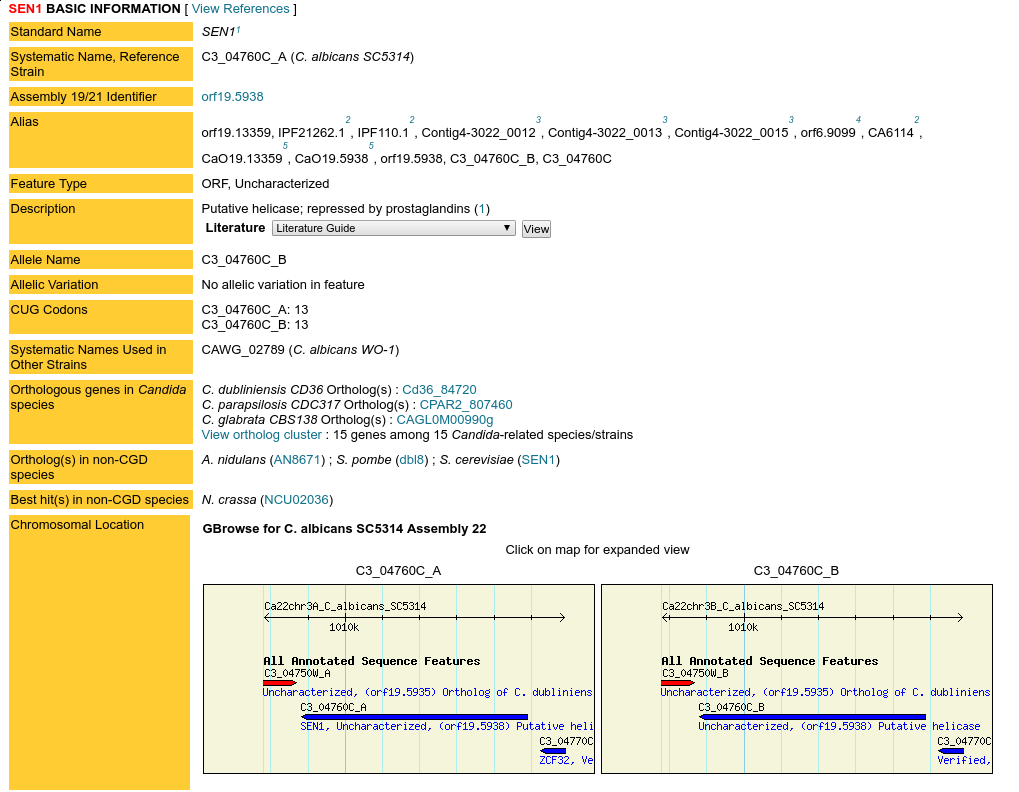
\includegraphics[scale=0.40]{cgd-locus}
\caption{Candida Genome Databases's locus page}
\end{center}
\end{figure}

Next the Yeast Genome\cite{sgd} project's locus page was inspected:

\begin{figure}[H]
\begin{center}
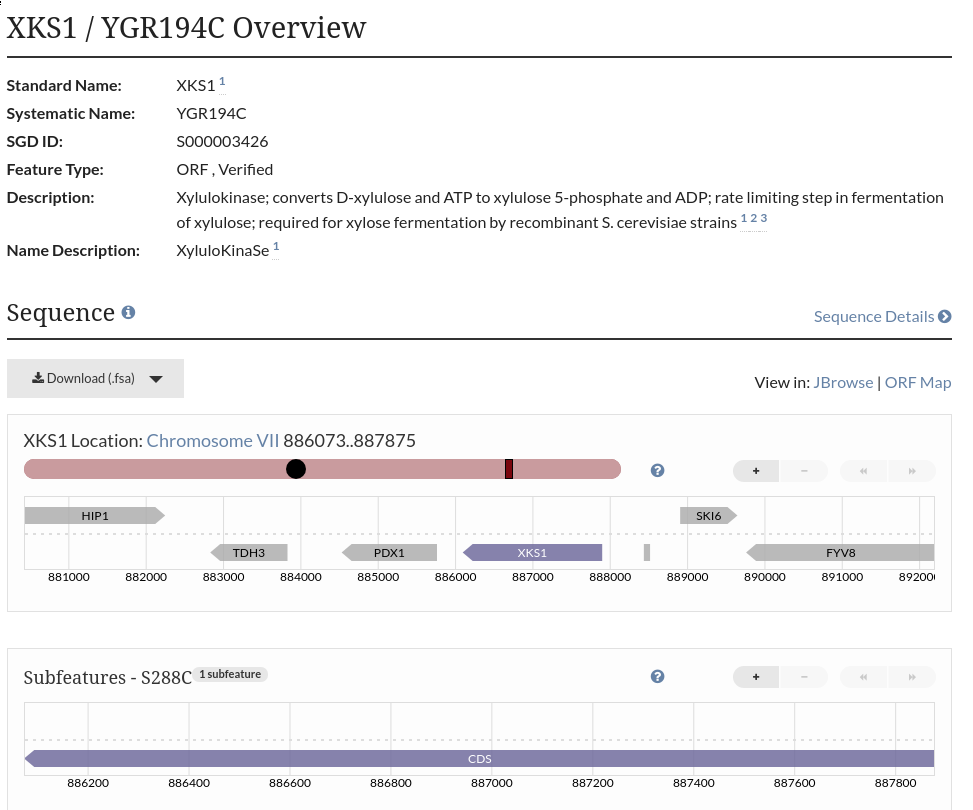
\includegraphics[scale=0.40]{sgd-locus}
\caption{Yeast Genome Project's locus page}
\end{center}
\end{figure}

This page was very nicely formatted and laid out, it clearly had a lot of development, as it had integrations with two genome browsers as well as a large amount of extra information and graphical representations of the genes locations. Replicating this would be ideal, however it is too far out of the scope of this project, as many extra systems would have to be setup to get this data and make it as interactive.

Much like the rest of this project the UI was prototyped along with the understanding of the data at the time. This means that the UI was evolving with the data, and wasn't truly decided upon and polished until the data that was being displayed was known to be correct, and wouldn't change. Unfortunately this didn't happen until quite late in the project. 

\subsubsection{Final design}
The focus for this design was to make it as simple to implement and use as possible, as this isn't a public facing service it doesn't need to be a cutting edge design aimed at grabbing users attention. Instead it just needs to be functional and represent the data clearly. 

There are only two main pages on the website, a search view, and a locus page for specific genes. These share the same template, and adapt based on the data provided to them. The tasks for these pages are simply to display the data in the database, and provide a form to query it.

Tooltips were used to display information about each row. As the site is only going to be used by a couple of researchers there wasn't much benefit to creating a help section or a how to guide on how to use the site, as firstly it has been changing a lot during development and secondly it is quicker to just have a direct conversation with them about areas that they might not understand. However if in the future this were to become a public service, I would create an extra information page that lists more background information about the project, the data and how the website is to be used. 

The page was constructed with bootstrap's\cite{bootstrap} grid system, which allows the content to be dynamically repositioned to fit different size displays.

\begin{figure}[H]
\begin{center}
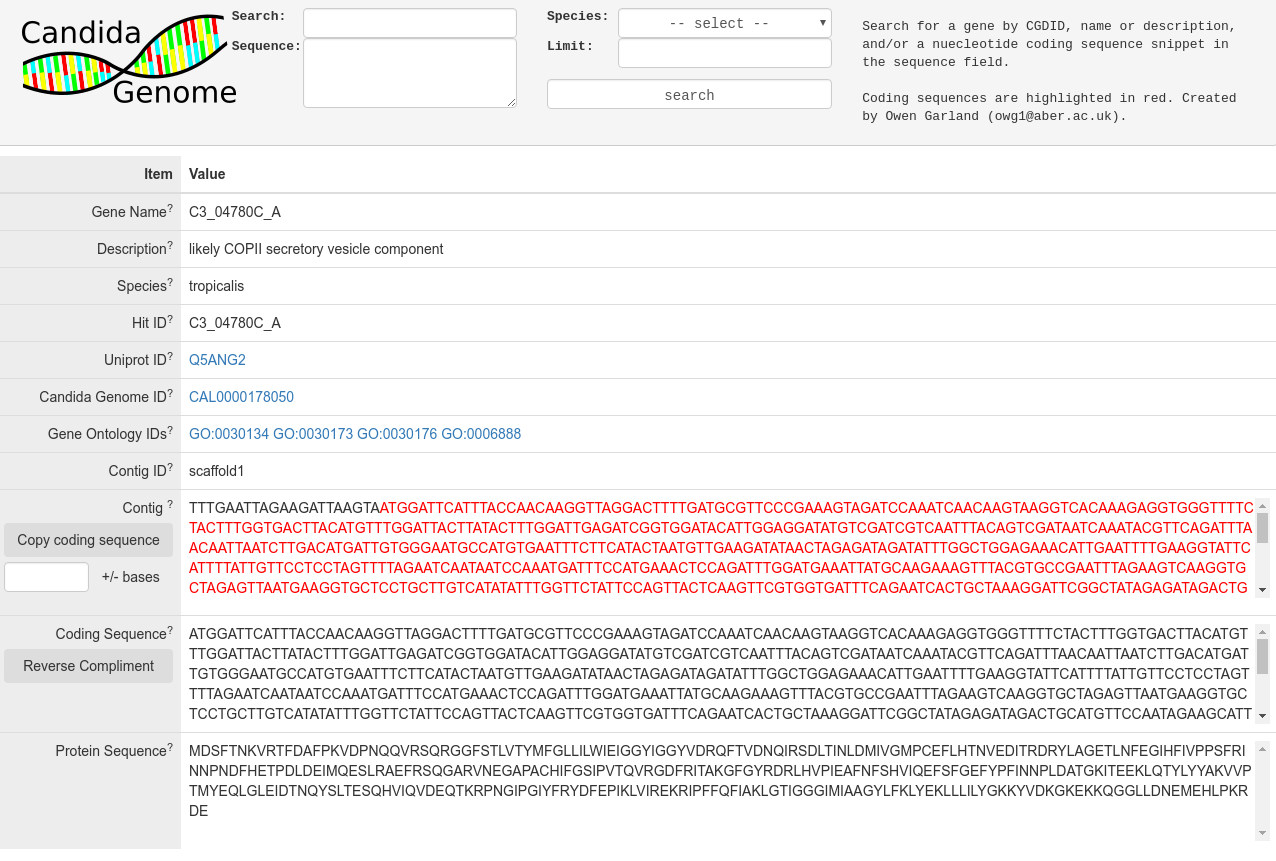
\includegraphics[scale=0.30]{candida-locus}
\caption{The final locus page for the project}
\end{center}
\end{figure}

\begin{figure}[H]
\begin{center}
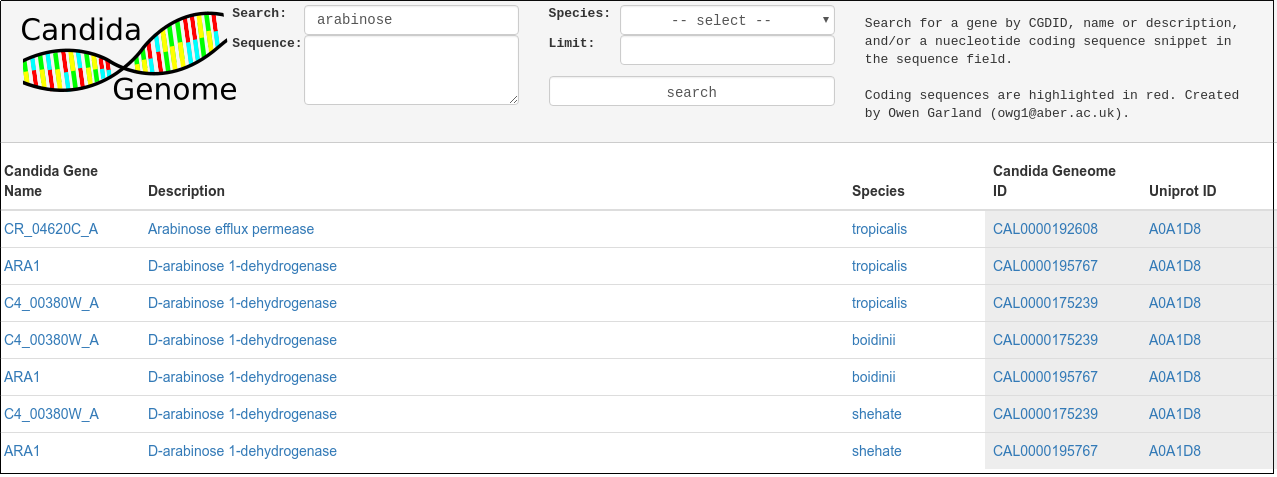
\includegraphics[scale=0.35]{candida-search}
\caption{The final search page for the project}
\end{center}
\end{figure}

\begin{figure}[H]
\begin{center}
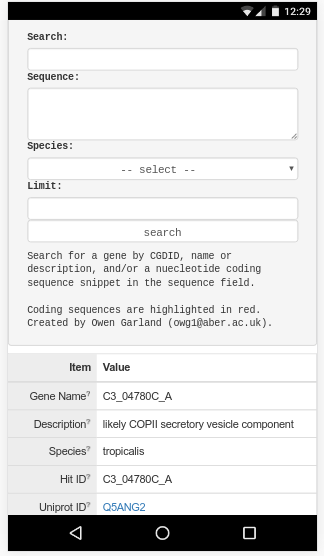
\includegraphics[scale=0.6]{candida-mobile}
\caption{A locus page viewed on a mobile device}
\end{center}
\end{figure}

\begin{figure}[H]
\begin{center}
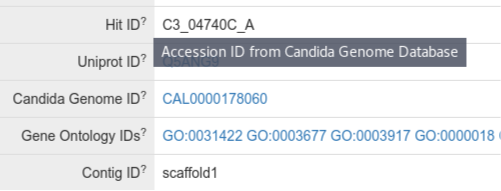
\includegraphics[scale=0.6]{candida-tooltip}
\caption{Tooltip on mouse hover describing what row means}
\end{center}
\end{figure}

\section{Implementation}
During the investigation into the data, many issues were encountered. Mainly due to a lack of understanding of what the data meant, and how it was produced. Initially the plan was to take the raw contigs for each species and use diamond to align them against the NCBI nr database. Then from those results link the data back to the Candida Genome Database via the RefSeq ID's that the NCBI nr database uses. However it was later discovered that there was an annotated set of blast data in the provided data, meaning that this step was no longer necessary.

A prototype was built around this blast data, however it was then realised that the data for \textit{C. boidinii} was not aligned against the NCBI nr database, but rather another unknown data set. This meant that to pursue this line of prototyping a replacement dataset for \textit{C. boidinii} would have to be made, or reproduce all three with another pipeline, as the results from the alignments weren't consistent. 

The core problem was that it was unknown what tools had been used to produce this data as there was no accompanying documentation. It appeared that a proprietary tool blast2go\cite{blast2go} had been used to align and annotate the data. However after using a trial copy to try and replicate the results it was evident that this tool had not actually been used to create the alignments with the NCBI nr database. 

Eventually it became clear that the alignment had just been performed with the BLAST tool, on the universities high performance cluster, with an XML format that wasn't known to have been an options at the time. This meant that the data could actually be reproduced quite easily with Diamond, using the newly discovered XML output that BLAST offers.

After these revelations, and another meeting with the researchers, we discovered in the original datasets that there were in fact already annotated protein sequence files and coding sequence files.

\subsection{Collating the data, and linking it to Candida Genome Database}
This meant that the data was already processed and largely annotated already. There was however one missing piece which was the link back to the Candida Genome Database (CGD), something that would be invaluable to the researchers who were already familiar with the CGD. 

Because of this, thankfully the weeks of effort spent learning about alignments and annotations weren't wasted, as a new alignment was needed to be produced, the coding sequences in the data set against the proteins found in \textit{C. albicans}, the latter being provided by CGD\cite{albicans}. 

This data generated was then able to be used to link the coding sequences found in our data sets to the well documented genes in \textit{C. albicans}. In addition to this the other annotations provided by the original dataset, such as Gene Ontology ID's, are able to be enhanced by using a mapping from the Candida Genome Database to get UniprotKB ID's which offer even more information on the known genes. 

Now each species had, the raw assembled contigs, the coding sequences, the amino acid sequences, the annotated protein information, a link to the Candida Genome Database, and in some cases a link to the UniprotKB database.


\subsection{Finding the coding sequence in the contig}
The next key piece of information to recover that would be of great use to the researchers was the position of the gene (coding sequence) inside the raw assembled contig. With this information they would be able to easily find the sequence of bases that surround the gene.

To do this mock data was produced manually, that contained the correct results, and unit tests made to check if a dummy function was returning the correct results as defined in the mock data. Then an algorithm was developed to find the position of a coding sequence inside a contig. 

The initial algorithm was only finding around fifty percent of the genes in the dataset. After some discussions with my supervisor, it became apparent that the reason for this is that the coding sequences were stored "in one direction", but the alignment results were finding genes that were the reverse compliment of that. This explains why around fifty percent of the genes weren't found. 

Modifying the algorithm to search for the reverse compliment of the coding sequence if it wasn't found "the first way", resulted in every gene being detected. The algorithm, simply found the index of the first twelve bases of the coding sequence in the contig, and the last twelve bases of the coding sequence in the contig. If the start or end couldn't be found it was assumed that the gene was spread across two contigs and the start or end respectively were marked to indicate that the gene was split across two contigs. 

\begin{figure}[H]
\begin{center}
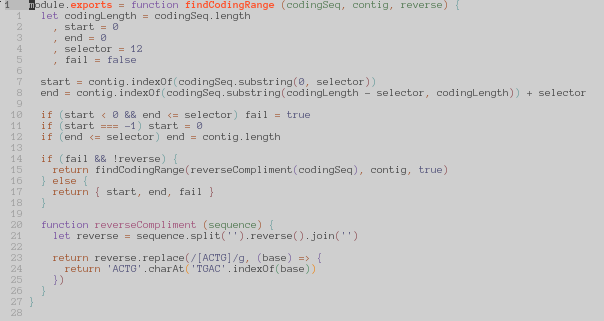
\includegraphics[scale=0.70]{code4}
\caption{Algorithm to find coding sequence inside a contig. \label{overflow}}
\end{center}
\end{figure}

\subsubsection{Search functionality}
Implementation of the search feature underwent several iterations, initially a search based on a regex match was implemented. This meant that each field was searched individually for any subset of the query string. This was very powerful as it would allow substrings to be found for each property of the searched for term. 

An example of this would be if `glucose-6' was searched in the description field, all documents in the database with that string in the description would be returned. This could then be combined with other fields to narrow down the query. 

This implementation was done during the prototyping phase to get a very basic search working for testing purposes, the reason it wasn't going to remain in the application is that a project wide regex search is very inefficient as the search has to be matched against every value int eh entire database for every single query made. Something that would have slowed down the site to unusable levels of performance.

A better solution was to create a generic search field using MongoDB's textSearch\cite{textsearch} feature, that utilises pre-compiled indexes to lookup data in a much more advanced manner. Indexing is quite an intensive task, however for this application where the data is only being read from the service, there is only a need to generate an index once, when the data is being imported to the database, this means the negative impact of an index isn't really in effect, as the import stage is a one time event. 

The fields indexed for the text search are the gene name, protein description, Uniprot ID and Candida Genome ID. Weights are then applied to each field to determine their value when sorting the results of a search. For example a match with a Uniprot ID is weighted higher than a protein description, allowing for results that have a match to a Uniprot ID are sorted higher than those without.  

With this system in place the search was functioning very well, however there was an issue, if a search returned a large amount of documents back, the sort was unable to be ran due to the default MongoDB sort buffer limit. To get around this issue the search function was re-written as an aggregate function. Aggregate\cite{aggregate} in MongoDB allows for a pipeline of steps to be applied to a query, as well as the option to use disk if memory limits are reached. 

\begin{figure}[H]
\begin{center}
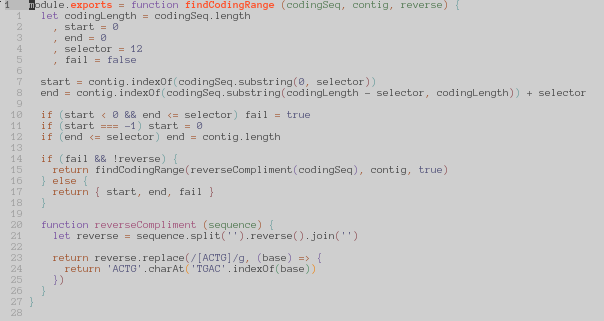
\includegraphics[scale=0.60]{code4}
\caption{Function responsible for creating the aggregate search query. \label{overflow}}
\end{center}
\end{figure}


% This section should discuss issues you encountered as you tried to implement your experiments. What were the results of running the experiments? What conclusions can you draw from these results? 
% 
% During the work, you might have found that elements of your experiments were unnecessary or overly complex; perhaps third party libraries were available that simplified some of the functions that you intended to implement. If things were easier in some areas, then how did you adapt your project to take account of your findings?
% 
% It is more likely that things were more complex than you first thought. In particular, were there any problems or difficulties that you found during implementation that you had to address? Did such problems simply delay you or were they more significant? 
% 
% If you had multiple experiments to run, it may be sensible to discuss each experiment in separate sections. 

\section{Testing}
Initially it was planned to develop this application in a test driven manner, as it leads to high quality code and stable solutions. 

The difficulty with this approach was that when developing prototypes rapid development is key, as it allows you to try out many different solutions. If a strict TDD pattern was followed during this phase the prototyping would have been drastically slowed as the amount of development work would have doubled. Unfortunately this wasn't a worthy endeavour as time was limited and developing tests for prototype code that may never end up in the final codebase was not going to be feasible.

Another difficulty in testing this project was that the majority of the projects logic is in the seed script that imports the data into the database. Testing this would be difficult because the only way of really checking the validity of what it was producing was to look at what was in the database and to see if that made sense in a biological context. 

Unfortunately it would be beyond the scope of this project to test the biological accuracy of the data that was imported. However I was able to manually verify that the data was correct at several stages, by aligning sequences from this project against other genomic databases such as the Candida Genome Database\cite{cgd} and the Yeast Genome\cite{sgd} project. 

\subsection{Automated Testing}
For the area's of logic that were testable, a TDD design was followed, mainly for the selection of the coding sequence in the contig, as this was the only real area of logic in the project that had it's own custom algorithm to be tested. In addition to this the test suite that was being used for the project also checked the project for code formatting issues with the eslint\cite{eslint} tool. This will cause the tests to fail if potentially dangerous assertions are made in the code. For example if a `==` was used instead of a `===` it will throw and error highlighting the issue to the developer. 

\subsubsection{Unit Tests}
Where possible test driven development was used to produce unit tests, these were mainly written for the logic that detects the coding sequence inside the contig. This is a crucial algorithm as the sites functionality depends on this data being accurate, so it was important that the algorithm be thoroughly tested. To do this several mock database records were created that had all the different possibilities that a gene could be found in, a normal hit, a reverse compliment hit, a missing hit and a hit that was split above and below the contig. 

Tests were then written to compare the result of the finding function against the correct values stored in the mock data. You can see this in the file `find-coding-range.test.js' where the tests are located. The function was then able to be developed ensuring that the data it was returning was correct. 

\subsection{User Interface Testing}
The user interface hasn't had automated tests written for it unfortunately, as there was only one HTML page and only two sets of data that were being returned it didn't feel particularly necessary to write tests to check that the data was coming through correctly. 

That being said the UI has been manually tested on Chrome, Firefox and Internet Explorer to check for any functional issues. None were found, however it was noted that in Internet Explorer there was some font rendering issues, but this isn't a concern as it doesn't impact the functionality of the site. I will be recommending that the site is used on Chrome though, as that it was it was developed on, so is the most thoroughly tested. 

Once the site was at a stage where it could be demonstrated the UI was shown to the researchers and they were asked to provide any feedback that might make the site easier to use for them. This feedback was.... yaydadada .... because of this feedback xyz was done to make it abc for them to use.

\subsection{Stress Testing}
As this site is hosting commercially sensitive data, it won't be publicly accessible, this means that only the researchers who are working on this data will be accessing it. Because of this there isn't a need to perform any stress testing on the service, as the stack is more than capable of handling < 10 users at a time, and isn't vulnerable to public attacks. 

\subsection{Integration Testing}
As listed in the build process section 3.2.4, continuous integration services were used throughout this project, meaning that every time a new build was pushed to github, it had to pass tests on the CI server before being deployed to the production server. This has ensured that any modifications to the code base won't break the core functionality of the production build. 

\subsection{User Testing}
Once the site has been developed to a stage where the users can get a real sense of how it is looking and how it will function, they have been invited to suggest changes that need to be made, in line with the agile practices that this project has been developed with. 

User testing was invaluable as the researchers were able to spot mistakes in the biological data that were invisible to the developer. An instance of this is when they noted that one of the UniprotID's was linking to a gene found in the Flu virus, something that shouldn't be present at all in the yeast genome. After investigating it was found that some of the UniprotID's has been truncated which caused this anomaly. Writing tests for these kinds of checks would have been nigh on impossible, thankfully user tests were able to pick up these kinds of issues. 

% Detailed descriptions of every test case are definitely not what is required here. What is important is to show that you adopted a sensible strategy that was, in principle, capable of testing the system adequately even if you did not have the time to test the system fully.

% Provide information in the body of your report and the appendix to explain the testing that has been performed. How does this testing address the requirements and design for the project?

% How comprehensive is the testing within the constraints of the project?  Are you testing the normal working behaviour? Are you testing the exceptional behaviour, e.g. error conditions? Are you testing security issues if they are relevant for your project? 

% Have you tested your system on ``real users''? For example, if your system is supposed to solve a problem for a business, then it would be appropriate to present your approach to involve the users in the testing process and to record the results that you obtained. Depending on the level of detail, it is likely that you would put any detailed results in an appendix.

% The following sections indicate some areas you might include. Other sections may be more appropriate to your project. 

\chapter{Deployment}


\section{User feedback}
Once the application had been through several development iterations and was nearing completion, it was presented to the researchers for signing off, discussions about deployment and maintenance provisions. Only one major change was requested, to have the site password protected, as they wanted to restrict access to only trusted researchers working on the project, until the research was published.

Ideally a password system would allow for multiple users with different passwords, with some levels of account controls by an administrator. This would be quite an extensive bit of work to undergo as a new users model would have to be created and the user interface would have to be updated to reflect all of the these new controls. Due to the time restrictions on this project, this was not a feasible request to complete to a satisfactory level.

An alternative, but far inferior solution was instead implemented, simply adding a Basic HTTP Auth header to the application. This involved only adding a module (basic-auth-connect) to the application, and one line of code to enable it in the middleware of the app. This does provide a password protection to the site to keep curious eyes out of the project, however it is very insecure as the password is stored on the server in plain text, as well as transmitted unencrypted over HTTP, since HTTPS hasn't been implemented for this service. 

\section{Deployment}
To deploy this project, an Ubuntu 16.04 Virtual Machine (VM) with three cores, 10GB of storage and 4GB of RAM was provisioned by the university. A user `candida' was then made for the project to be ran under and the release branch of the project cloned down to the machine from the Github repository. Node.js was then installed from the Ubuntu repositories, so that the system had access to the Node Package Manager (npm). This was then used to install nave\cite{nave}, m\cite{m}, and yarn\cite{yarn}. Three tools that help with the management of packages and versioning for Node.js, MongoDB and npm packages.

Nave was then used to install Node.js version 6.9.0, which is what this application was developed for, and m was used to install MongoDB 3.4.4. The dependencies listed in the package.json file were then installed to the node\_modules folder with yarn, the project could then be build with the build script defined in the package.json. This process is documented in the projects README.md file.

To generate the data for the database and import it to MongoDB, the seed script defined in the package.json was run, this runs the importation script using the data that is included in the repository to populate the database.

To ensure the stability of the service, it was put behind a Varnish\cite{varnish} cache. Doing this enabled caching on all of the responses from the web server to client requests, meaning that if a request has already had a response processed for it, then a cached version will be served from Varnish rather than adding load to the Node.js application. This speeds up the sites response time as data can be immediately returned, once it has been processed already.

Unfortunately a side effect of the last minute need to include basic HTTP auth, is that the benefits from puttin ghte service behind Varnish are nullified, as Varnish won't cache content behind a basic HTTP auth. This another good reason to find a better solution to the password protection in the future.

A systemd\cite{systemd} service file was then written and installed on the server for the Node.js process, this enables the application to be controlled from systemd. This is done so that the application can be started at boot time, as well as monitored, restarted and stopped from the systemd interface; which is how all the other services on the VM are controlled.

One difficulty faced during this deployment was the versioning on MongoDB, provided by the OS on the VM. The application had been developed on Arch Linux which provides a recent version (3.4) of MongoDB in it's package manager, however on the VM which was running Ubuntu, the package was for version 2.6, that doesn't support the new wiredTiger\cite{tiger} storage engine. 

The difference in versions was noted initially, and corrected by installing version 3.4. However when data was entered into the database, it was taking up around three times as much room, filling up the VM's disk space. 

To correct this a manual process of updating the storage engine and database directory in the MongoDB configuration was necessary. This enabled the data to be imported correctly, taking up the expected amount of storage. 

With the deployment complete, the README.md file in the project was updated to reflect the steps necessary to replicate a full deployment, so that other developers could replicate the production environment. 

\chapter{Evaluation}

% Examiners expect to find in your dissertation a section addressing such questions as:

\begin{itemize}
   \item Were the requirements correctly identified? 

     Part of the difficulty of this project was going through several iterations of understandings of the data, and how it needed to be interpreted. This meant that the requirements only really became clear very late in the project. However once they were apparent, development from then on was very straight forward. 

   \item Were the design decisions correct?

     The project is functional, and hasn't suffered any bugs, and meets all of the achievable criteria so I believe the design decisions were correct.

   \item Could a more suitable set of tools have been chosen?

     The use of NodeJS and MongoDB does set this project apart from older similar projects, that use Perl and PostgreSQL. However there is a clear shift in the technologies used for web development, as Perl is on the decline\cite{needed}, and newer technologies like NodeJS are taking it's place. The advantages presented to a web developer of NodeJS are clear and outlined in the design choices section. 

   \item How well did the software meet the needs of those who were expecting to use it?

     Hopefully will find out on Friday!

   \item If you were starting again, what would you do differently?

     Try to talk to the source of the data sooner and ideally schedule a session with the researchers to look over the data and hopefully unpick what it all meant a lot sooner than we did. 
\end{itemize}

% Other questions can be addressed as appropriate for a project. 

% Such material is regarded as an important part of the dissertation; it should demonstrate that you are capable not only of carrying out a piece of work but also of thinking critically about how you did it and how you might have done it better. This is seen as an important part of an honours degree. 

I'm very pleased with the end result of the project, it is a nicely developed clean piece of software that meets it's basic functional requirements. The area that really could have been improved upon was the amount of time it took to get to grips with the data. If I had had the understanding of it much earlier in the project, there could have been more features developed that would have helped the researchers a lot more than what I was able to produce. One area that I would have loved to be able to explore was creating a comparison tool, which would allow them to compare two or more genes directly. 

This would have added a lot more complexity to the project, but considering how smoothly the development of the application went, once the data was understood correctly, I think there would have been plenty of time. The actual development of the database and website did only take around a week, so there was a lot more room for new features, had the data been understood earlier. 

% There will be good things and room for improvement with any project. As you write this section, identify and discuss the parts of the work that went well and also consider ways in which the work could be improved. 

The application was built with very robust software engineering principles, and the code is a testament to how cleanly it was developed, there are very few code smells\cite{smells} throughout the code. This is mostly thanks to the discipline enforced by having linters and automated testing. The only area that falls down in this regard is the amount of unit tests. As the project stands there are only a handful of unit tests to check the finding of coding sequences. Ideally it would be good to expand the testing to cover the Pug templates, the controller logic, and the search functionality. 

Unfortunately by the time the data was understood enough to develop the application fully, there was not enough time to test these features and write up this report. 

In the future this will be deployed to the university servers, and I will offer to help maintain and develop new features for the researchers if they need it, as I am keen for their project to go well, which what provided the motivation for this project to be a success, which overall I feel that it has been. 

% add any additional chapters here

\setemptyheader
\addcontentsline{toc}{chapter}{Appendices}
\chapter*{Appendices}
The appendices are for additional content that is useful to support the discussion in the report. It is material that is not necessarily needed in the body of the report, but its inclusion in the appendices makes it easy to access. 

For example, if you have developed a Design Specification document as part of a plan-driven approach for the project, then it would be appropriate to include that document as an appendix. In the body of your report you would highlight the most interesting aspects of the design, referring your reader to the full specification for further detail.

If you have taken an agile approach to developing the project, then you may be less likely to have developed a full requirements specification. Perhaps you use stories to keep track of the functionality and the 'future conversations'. It might not be relevant to include all of those in the body of your report. Instead, you might include those in an appendix. 

There is a balance to be struck between what is relevant to include in the body of your report and whether additional supporting evidence is appropriate in the appendices. Speak to your supervisor or the module coordinator if you have questions about this.

\pagebreak

% start the appendix - sets up different numbering
\fancypagestyle{plain}{%
%\fancyhf{} % clear all header and footer fields
\fancyhead[L]{\textsl{Appendix\ \thechapter}}
\fancyhead[R]{\textsl{\leftmark}}}

\appendix
\fancyhead[L]{\textsl{Appendix\ \thechapter}}
\fancyhead[R]{\textsl{\leftmark}}
\fancyhead[C]{}
\fancyfoot[C]{\thepage}
\renewcommand{\headrulewidth}{0.4pt}
\renewcommand{\chaptermark}[1]{\markboth{#1}{}}

\fancyhead[L]{\textsl{Appendix\ \thechapter}}
\fancyhead[R]{\textsl{\leftmark}}
\fancyfoot[C]{{\thepage} of \pageref{LastPage}}

% include any appendices here
\chapter{Third-Party Code and Libraries}
\section{Nodestack}

\url{https://github.com/bag-man/nodestack}

This project uses boilerplate code developed by myself for previous projects. The code sets up a basic Node JS project, with access to to third party services. During the development of this project some features were merged back into the boilerplate, such as the mongoose integration.  This boilerplate makes use of several third party libraries, which are all listed in the package.json. Some extra modules have also been added specific to this project such as fasta2json and the clipboard module. 

\section{Externally hosted libraries}
\subsubsection*{JQuery} 

\url{https://github.com/jquery/jquery} - MIT

JQuery is a client side javascript library that makes navigating and interacting with the HTML DOM far easier. 

\subsubsection*{Bootstrap} 

\url{https://github.com/twbs/bootstrap} - MIT

Bootstrap is a library for styling webpages and making them easily responsive to different screen sizes.

\section{package.json}
Below is the modules listed in the package.json for the project, which can be found with the source code, all third party software is listed here along with it's version. This is how node modules are packaged, this automates the management of all modules, and locks the versions. For this project I was using yarn\cite{yarn} to manage the packages rather than the default node package manager (npm)\cite{npm}. Yarn has a couple of advantages, mainly that it is a lot faster than npm3 and that it automatically creates a lock file for modules and their dependencies. 

\subsection{Development Dependencies}
  This section of third party modules are not installed on the production builds of the application, they are only for use when developing the application, they don't change the functionality of it at all, just make it easier to work on. 

\subsubsection*{codecov} 

\url{https://www.npmjs.com/package/codecov} @ 1.0.1 - MIT

This provides integration with codecov's services, to provide interactive test coverage information.

\subsubsection*{basic-auth-connect} 

\url{https://www.npmjs.com/package/basic-auth-connect} @ 1.0.0 - MIT

This provides a basic HTTP auth middleware for express.

\subsubsection*{eslint}  

\url{https://www.npmjs.com/package/eslint} @ 2.3.0 - MIT

This is the linting engine that is used to check the source code for mistakes.

\subsubsection*{eslint-config-clock} 

\url{https://www.npmjs.com/package/eslint-config-clock} @ 1.2.0 - ISC

This is a set of configurations for eslint that describe the code formatting that is preferred for this project.

\subsubsection*{eslint-config-standard} 

\url{https://www.npmjs.com/package/eslint-config-standard} @ 5.1.0 - MIT

The clock config is built on top of this standard configuration

\subsubsection*{eslint-plugin-promise} 

\url{https://www.npmjs.com/package/eslint-plugin-promise} @ 3.3.0 - ISC

Eslint didn't support promises natively at the time of writing, so this was used to detect promises in the code.

\subsubsection*{eslint-plugin-standard} 

\url{https://www.npmjs.com/package/eslint-plugin-standard} @ 1.3.1 - MIT

Add's a few extra rules to eslints configuration options.

\subsubsection*{husky} 

\url{https://www.npmjs.com/package/husky} @ 0.13.2 - MIT

Simply runs the test suite before code is pushed to remote repositories.

\subsubsection*{istanbul} 

\url{https://www.npmjs.com/package/istanbul} @ 1.0.0-alpha.2 - BSD-3-Clause

Provides coverage information at the end of the test suite, and for codecov's usage.

\subsubsection*{mocha} 

\url{https://www.npmjs.com/package/mocha} @ 3.1.2 - MIT

Testing framework for javascript.

\subsubsection*{nodemon} 

\url{https://www.npmjs.com/package/nodemon} @ 1.11.0 - MIT

Monitors source files for changes, and relaunches the application when files are changed.

\subsection{Build Dependencies}
These third party modules are the frameworks libraries and modules that are actually used to by the application to function. 

\subsubsection*{babel}

\url{https://www.npmjs.com/package/babel} @ 7.5.2 - MIT

Transpiler for javascript. Used for converting ES6 code into ES5 for browser compatibility.

\subsubsection*{babel-core}

\url{https://www.npmjs.com/package/babel-core} @ 6.18.0 - MIT

Core configurations for babel.


\subsubsection*{babel-loader}

\url{https://www.npmjs.com/package/babel-loader} @ 6.2.5 - MIT

Allows for transpiling to be done from webpack build manager.

\subsubsection*{babel-preset-es2015}

\url{https://www.npmjs.com/package/babel-preset-es2015} @ 6.18.0 - MIT

The standard ES5 configuration.

\subsubsection*{clipboard}

\url{https://www.npmjs.com/package/clipboard} @ 1.6.1 - MIT

Clipboard module used for copying text to a users system clipboard from the browser.


\subsubsection*{express}

\url{https://www.npmjs.com/package/express} @ 4.14.0 - MIT

The web framework that powers the node application.

\subsubsection*{fasta2json}

\url{https://www.npmjs.com/package/fasta2json} @ 0.1.1 - MIT

Module that reads fasta files into JSON objects.

\subsubsection*{mongoose}

\url{https://www.npmjs.com/package/mongoose} @ 4.8.6 - MIT

MongoDB object modelling framework.

\subsubsection*{morgan}

\url{https://www.npmjs.com/package/morgan} @ 1.7.0 - MIT

Cleaner and clearer logging output.

\subsubsection*{pug}

\url{https://www.npmjs.com/package/pug} @ 2.0.0-beta11 - MIT

HTML templating language.

\subsubsection*{stylus}

\url{https://www.npmjs.com/package/stylus} @ 0.54.5 - MIT

CSS templating language.

\subsubsection*{webpack}

\url{https://www.npmjs.com/package/webpack} @ 2.2.1 - MIT

Javascript build manager.


% If you have made use of any third party code or software libraries, i.e. any code that you have not designed and written yourself, then you must include this appendix. 

% As has been said in lectures, it is acceptable and likely that you will make use of third-party code and software libraries. If third party code or libraries are used, your work will build on that to produce notable new work. The key requirement is that we understand what is your original work and what work is based on that of other people. 

% Therefore, you need to clearly state what you have used and where the original material can be found. Also, if you have made any changes to the original versions, you must explain what you have changed. 

% As an example, you might include a definition such as: 

% Apache POI library - The project has been used to read and write Microsoft Excel files (XLS) as part of the interaction with the client's existing system for processing data. Version 3.10-FINAL was used. The library is open source and it is available from the Apache Software Foundation 
% \cite{apache_poi}. The library is released using the Apache License 
% \cite{apache_license}. This library was used without modification. 

\chapter{Ethics Submission}

This appendix includes a copy of the ethics submission for the project. After you have completed your Ethics submission, you will receive a PDF with a summary of the comments. That document should be embedded in this report, either as images, an embedded PDF or as copied text. The content should also include the Ethics Application Number that you receive. 
\chapter{Code Examples}

% For some projects, it might be relevant to include some code extracts in an appendix. You are not expected to put all of your code here - the correct place for all of your code is in the technical submission that is made in addition to the Final Report. However, if there are some notable aspects of the code that you discuss, including that in an appendix might be useful to make it easier for your readers to access. 
% 
% As a general guide, if you are discussing short extracts of code then you are advised to include such code in the body of the report. If there is a longer extract that is relevant, then you might include it as shown in the following section. 
% 
% Only include code in the appendix if that code is discussed and referred to in the body of the report. 



\fancypagestyle{plain}{%
   \fancyhead{} %[C]{Annotated Bibliography}
   \fancyfoot[C]{{\thepage} of \pageref{LastPage}} % except the center
   \renewcommand{\headrulewidth}{0pt}
   \renewcommand{\footrulewidth}{0pt}
}

\setemptyheader

\nocite{*} % include everything from the bibliography, irrespective of whether it has been referenced.

% the following line is included so that the bibliography is also shown in the table of contents. There is the possibility that this is added to the previous page for the bibliography. To address this, a newline is added so that it appears on the first page for the bibliography. 
\addcontentsline{toc}{chapter}{Annotated Bibliography} % Adds References to contents page

%
% example of including an annotated bibliography. The current style is an author date one. If you want to change, comment out the line and uncomment the subsequent line. You should also modify the packages included at the top (see the notes earlier in the file) and then trash your aux files and re-run. 
%\bibliographystyle{authordate2annot}
\bibliographystyle{IEEEannotU}
\renewcommand{\bibname}{Annotated Bibliography} 
\bibliography{References/references} % References file


\end{document}
